\chapter*{State, Actions, Observations, and Reward}
\label{sec:problem}


% TODO: Page 38 of Improving Sequential Decision Making in Human-In-The-Loop Systems

\section{Problems}

\begin{enumerate}
    \item How to get transition and observation probabilities? Am I correct that these need to be given by Florian's model? How would this ever be known in the case of learning with real human drivers?
    \item Is the Markov assumption satisfied even though the driver's attentiveness does not depend on the previous state and action?
    \item What is known a priori?
    \begin{itemize}
        \item human's current action (assumption: no, for performance reasons)
        \item reward function
    \end{itemize}
\end{enumerate}

\newpage

\section{State}

The tracks will be round courses. Thus, there is no terminal state if everything goes well. If the car reaches an off-track position, however, the car is reset to be in the initial starting position again.\\

\begin{tabularx}{\textwidth}{@{}p{0.18\textwidth}>{\centering}p{0.22\textwidth}X@{}}
\toprule
\textbf{Name}           & \textbf{Measurement}          & \textbf{Description}                                           \\ \midrule

Gear \newline \textbf{(constant)} & \{$-1$, $0$, $1$,  \dots, $6$\} & Distance of the car from the start line along the track line. \textbf{Neither the human driver nor the agent can directly influence this with their actions.} \\ \midrule

RPM \newline \textbf{(constant)} & [0, $+\inf$) & Number of engine rotations per minute. \textbf{Neither the human driver nor the agent can directly influence this with their actions.} \\ \midrule

Speed \newline \textbf{(constant)}  & ($-\inf$, $+\inf$) (km/h) & Speed along the longitudinal axis of the car. \textbf{Neither the human driver nor the agent can directly influence this with their actions.} \\ \midrule

% Lift \newline \textbf{(constant)} & ($-\inf$, $+\inf$) (km/h) & Speed along the vertical axis of the car. Will be zero as we use completely flat terrain. \textbf{Neither the human driver nor the agent can directly influence this with their actions.} \\ \midrule

Side force & ($-\inf$, $+\inf$) (km/h) & Speed along the transverse axis of the car. This is directly influenced by the steering actions of both human driver and agent. \\ \midrule

Distance from start & [0, $+\inf$) (m) & Distance of the car from the start line along the track line. \\ \midrule

Angle          & [$-\pi$, $+\pi$] (rad) & Angle between car direction and track axis direction.  \\ \midrule

Lane position & ($-\inf$, $+\inf$)     & Horizontal distance between the car and the track axis. $0$ when the car is on the axis, $+1$ if the car is on the left edge of the track, and $-1$ if the car is on the right edge of the track. Greater numbers than $+1$ or smaller numbers than $-1$ indicate that the car is off-track. \\ \midrule

Driver attention & True / False & Whether the human driver is attentive or distracted.  \\ \bottomrule

\end{tabularx}

\section{Actions}

\begin{tabularx}{\textwidth}{@{}p{0.18\textwidth}>{\centering}p{0.22\textwidth}X@{}}
\toprule
\textbf{Name}           & \textbf{Measurement}          & \textbf{Description}\\ \midrule

\multicolumn{3}{@{}>{\centering}p{\linewidth}@{}}{\textit{In our simplified scenario, both the human driver and the agent can not accelerate, brake or switch gears.}} \\ \midrule

Steering         & [$-2$, $+2$] & The input to the car is generated by combining the agent's action with the human's steering action (see equation \ref{eq:steering}). For the car,  $-1$ means full right (159 degrees) and $+1$ means full left (21 degrees). A value greater than +1 or lower than -1 can effectively reverse an opposite action of the human driver. \\ \bottomrule
\end{tabularx}\\\\

\noindent The human driver and the agent share control of the steering wheel. The speed of the car is fixed and cannot be altered; neither by human driver nor agent. The steering input of the driver $\mathcal{A}_{steer}^{driver}$ and agent $\mathcal{A}_{steer}^{agent}$ are combined to ${A}_{steer} \in [-1, +1]$ using equation \ref{eq:steering}.

The agent needs to be able to fully counteract a distracted driver's actions. In the extreme case, while the car is in a curve, a distracted driver could steer into the opposite direction of the trajectory of the lane center. Thus, the car would not only diverge from the lane center but would even get off the road completely. The agent thus needs to reverse the driver's action in order to keep the car centered in the lane and follow the road curve. Therefore, we define the range for the agent's steering action as follows: $\mathcal{A}_{steer}^{agent} \in [-2, +2]$.

\begin{equation}
    \mathcal{A}_{\textrm{steer}} = \min(\, -1, \, \max(\, 1, \, (\mathcal{A}_{\textrm{steer}}^{\textrm{driver}} + \mathcal{A}_{\textrm{steer}}^{\textrm{agent}})\,)\,)
    \label{eq:steering}
\end{equation}

\section{Observations}

\begin{figure}[ht]
    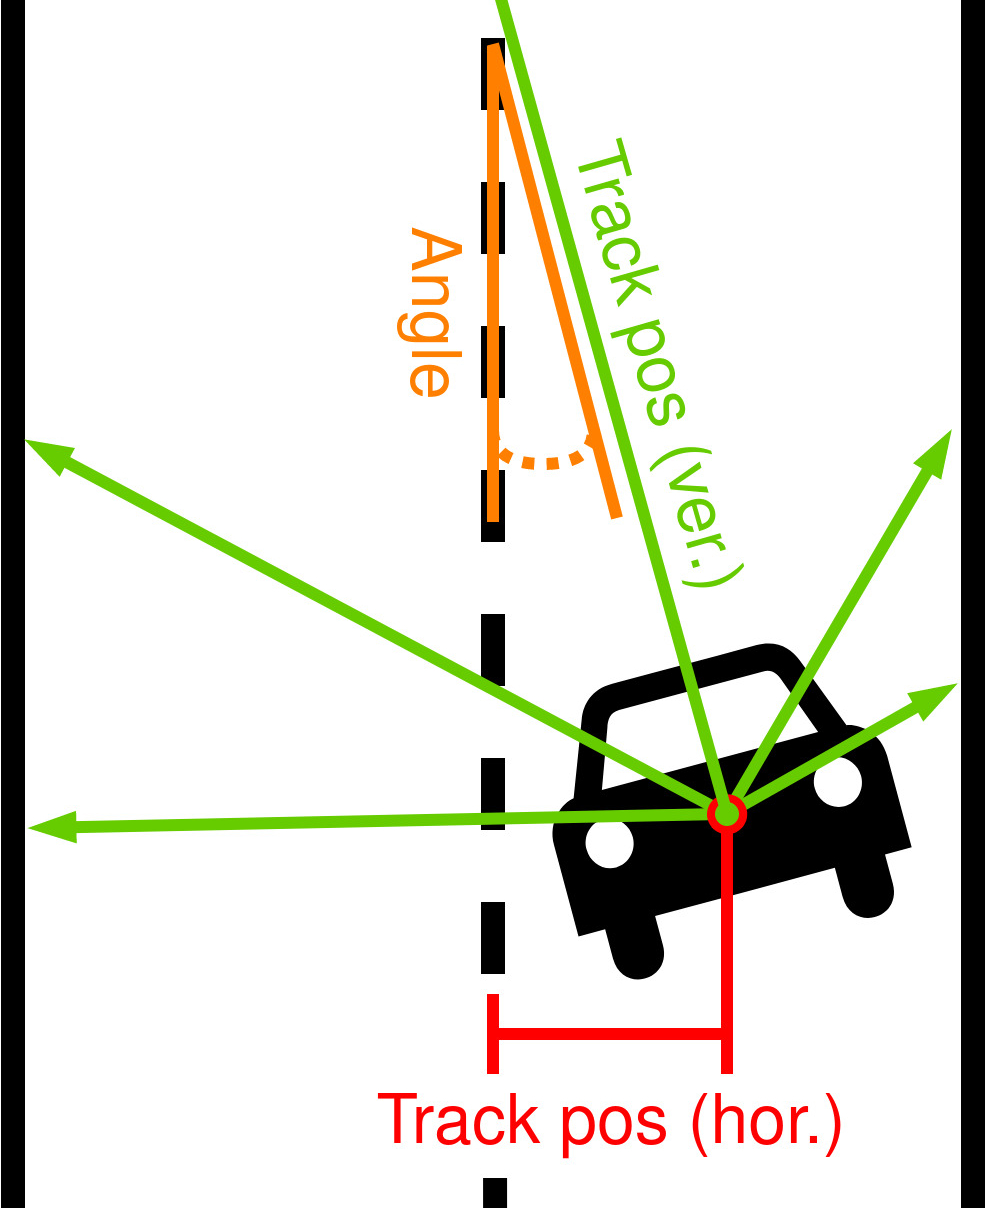
\includegraphics[width=0.3\linewidth]{figures/Observations.jpg}
    \centering
    \caption{Main environment observations}
    \label{fig:observations}
\end{figure}


\begin{tabularx}{\textwidth}{@{}p{0.18\textwidth}>{\centering}p{0.22\textwidth}X@{}}
\toprule
\textbf{Name}           & \textbf{Measurement}          & \textbf{Description}   \\ \midrule

\multicolumn{3}{@{}>{\centering}p{\linewidth}@{}}{\textit{Constant state parameters are not observed as they do not influence learning.} \textbf{The observations are not noisy.}} \\ \midrule

Angle          & [$-\pi$, $+\pi$] (rad) & Angle between car direction and track axis direction  \\ \midrule

Side force & ($-\inf$, $+\inf$) (km/h) & Speed along the transverse axis of the car. This is directly influenced by the steering actions of both human driver and agent. \\ \midrule

Track position (horizontal) & ($-\inf$, $+\inf$)     & Horizontal distance between the car and the track axis. $0$ when the car is on the axis, $+1$ if the car is on the left edge of the track, and $-1$ if the car is on the right edge of the track. Greater numbers than $+1$ or smaller numbers than $-1$ indicate that the car is off-track.  \\ \midrule

Track position (vertical)  & [$0$,$200$] (m) & Vector of 5 range finder sensors (of 19 available in TORCS). The range finders serve as lookahead by returning the distance between the car and the track edge in a given forward angle between $-90$ and $+90$ degrees with respect to the car axis. \\ \midrule 

Driver steering (last time step) & [$-1$, $+1$]  & The agent perceives the last input of the human. This is not the action of the human in the next but in the last time step. The agent does not know which action the human is going to choose simultaneous to its own action. $-1$ means full right (159 degrees) and $+1$ means full left (21 degrees).  \\ \bottomrule
\end{tabularx}

\newpage
\section*{Reward}

The overall goal for the agent is to only assist the driver in keeping the car centered in its lane. Therefore, this is the main source of reward for the agent. The more centered the car is at a certain time step, the more reward $r$ is received. However, the agent is supposed to leave the human driver with as much autonomy as possible. Thus, any intervention by the agent is penalized. Minor smooth interventions are generally preferred over large abrupt steering actions. Accordingly, the penalty is (exponentially) dependent on the intensity of the agent's action. The general assumption is that an attentive driver performs better in keeping the car centered than an inattentive driver. The agent has to predict whether a driver is attentive or not in order to choose its actions correctly. An incorrect prediction of the driver's actions will lead to overshooting and thus be negatively reflected in the reward for keeping the car centered. Lastly, the car is never supposed to leave the lane. Consequently, leaving the lane is highly penalized.


%For this reason, the penalty intensity is linked to the current distance of the car to the lane center; the higher the distance, the lower the agent's intervention penalty. On the other hand, 

% TODO: Add smoothing?

% \begin{equation}
%     \mathcal{R} = \mathcal{R}_{\textrm{center}} - \mathcal{P}_{\textrm{act position}} - \mathcal{P}_{\textrm{act intensity}} - \mathcal{P}_{\textrm{off-lane}}
% \end{equation}
\begin{equation*}
    \mathcal{R} = \mathcal{R}_{\textrm{center}} - \mathcal{P}_{\textrm{act intensity}} - \mathcal{P}_{\textrm{off-lane}}
\end{equation*}
\begin{equation*}
    \mathcal{R}_{\textrm{center}} = 
    \begin{cases}
        r - r * |Pos_{hor}| & \text{if} \quad |Pos_{hor}| \leq 1 \\
        0 & \text{if} \quad \text{off-lane}
    \end{cases}
\end{equation*}
% \begin{equation}
%     \mathcal{P}_{\textrm{act position}} = 
%     \begin{cases}
%         p_{\textrm{pos}} - p_{\textrm{pos}} * |Pos_{hor}| & \text{if} \quad |Pos_{hor}| \leq 1 \text{ and } \mathcal{A}_{\textrm{steer}}^{\textrm{agent}} \neq 0 \\
%         0 & \text{if} \quad \text{off-lane or no steering action}
%     \end{cases}
% \end{equation}
\begin{equation*}
    \mathcal{P}_{\textrm{act intensity}} = |\mathcal{A}_{\textrm{steer}}| ^ {p_{\textrm{int}}}
\end{equation*}
\begin{equation*}
    \mathcal{P}_{\textrm{off-lane}} = 
    \begin{cases}
        p_{\textrm{off}} & \text{if} \quad |Pos_{hor}| > 1 \\
        0 & \text{if} \quad |Pos_{hor}| \leq 1
    \end{cases}
\end{equation*}